\documentclass{article} % For LaTeX2e
\usepackage{nips15submit_e,times}
\usepackage{hyperref}
\usepackage{url}
\usepackage{graphicx}
%\documentstyle[nips14submit_09,times,art10]{article} % For LaTeX 2.09

\title{Using Recurrent Neural Networks on the WAY-EEG-GAL dataset}

\author{
Roman C.~Podolski
\\
%Technische Universit\"at M\"unchen\\
%Pittsburgh, PA 15213 \\
\texttt{roman.podolski@tum.de} \\
\And
Dominik Irimi \\
%Affiliation \\
%Address \\
\texttt{dominik.irimi@gmail.com} \\
\AND
Christoph Dehner \\
%Affiliation \\
%Address \\
\texttt{dehner@in.tum.de} \\
\And
Manuel Nickel \\
%Affiliation \\
%Address \\
\texttt{manuel.nickel@tum.de} \\
\And
Philipp Bergmann \\
%Affiliation \\
%Address \\
\texttt{philipp.bergmann@tum.de} \\
}

% The \author macro works with any number of authors. There are two commands
% used to separate the names and addresses of multiple authors: \And and \AND.
%
% Using \And between authors leaves it to \LaTeX{} to determine where to break
% the lines. Using \AND forces a linebreak at that point. So, if \LaTeX{}
% puts 3 of 4 authors names on the first line, and the last on the second
% line, try using \AND instead of \And before the third author name.

\newcommand{\fix}{\marginpar{FIX}}
\newcommand{\new}{\marginpar{NEW}}

\nipsfinalcopy % Uncomment for camera-ready version

\begin{document}


\maketitle

\begin{abstract}
The \emph{WAY-EEG-GAL} dataset is designed to allow testing of techniques to decode sensation, intention and action from scalp EEG recordings in humans who perform a grasp-and-lift task. In this paper we present our methodology to analyze the data and how we tackled the problem of classifying various stages of these tasks by using a RNN on EEG and EMG data. In particular we present particular findings in the EEG data and successes as well as pitfalls concerning the RNN runs.
\end{abstract}

\section{The dataset}
In order to allow for critical evaluations of the utility of EEG signals for prosthetic control of object manipulation, the \emph{Wearable interfaces for hAnd function recoverY - EEG - Grisp And Lift (WAY-EEG-GAL)} dataset was created. In particular, it can be used to inter alia examine at what degree it is possible to identify the intention to reach and grasp, hand positions and velocities or that the object's properties have unexpectedly changed. The data was collected during the course of a series of experiments in which twelve right-handed individuals, both male and female, were selected as participants. Each participant was seated at a desk with his hand resting on the table. An LED signaled the person to reach for a small object, grasp it using his index finger and thumb, lift it up a few centimetres, hold it for a brief moment and finally return the object as well as his hand to their intial positions. In this paper, we will from now on refer to this sequence of events and actions as a \emph{trial}. \\
Each participant then conducted $328$ such trials under slight but to the participant unpredictably changing circumstances. That is, the object's weight to be lifted was augmented through an electromagnet, resulting in weights of $165$, $330$ or $660 g$. Furthermore, the contact surface changed to be made of sandpaper, suede or silk. Depending on the specific trial, either only the surface, only the object's weight, both or none changed. In order to record kinematics, forces, muscle activations and brain activity, four types of sensors were used during the experiments. In particular, an electroencephalography (EEG) cap, illustrated in figure \ref{fig:eeg_setup}, with $32$ electrodes was used to record the brain activity during the trials, sampling at $500 Hz$. Furthermore, five electromyography (EMG) sensors, as depicted in figure \ref{fig:emg_setup}, were placed on the participant's right arm to measure muscle activity at a sample rate of $4 kHz$.\\
\begin{figure}
	\centering
	\begin{minipage}{0.5\textwidth}
		\centering
		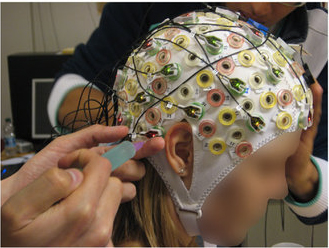
\includegraphics[width=1.0\textwidth]{images/eeg_setup.jpg}
		\caption{An EEG cap measures the participant's brain activity [1]}
		\label{fig:eeg_setup}
	\end{minipage}\hfill
	\begin{minipage}{0.49\textwidth}
		\centering
		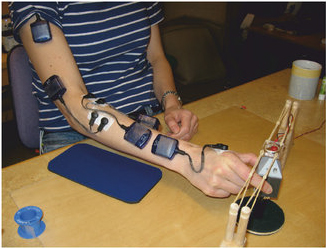
\includegraphics[width=1.0\textwidth]{images/emg_setup.jpg}
		\caption{EMG sensors record the muscle activity of the right arm [1]}
		\label{fig:emg_setup}
	\end{minipage}
\end{figure}
The resulting dataset, in the form that we used it, then provides the measurements for each participant and each trial. In this, the EEG and EMG signals are concatenated in matrices respectively with a time stamp decoding the exact record time for each measurement. Moreover, the time of the LED being turned on and off, the trial's start and end time, the type of surface and the object's weight are provided for each trial, as well. [1]


\subsubsection*{References}
 [1] Luciw, M. D., Jarocka, E., EdinLandsberger, B. B. (2014) Multi-channel EEG recordings during 3,936 grasp and lift trials with varying weight and friction. Retrieved July 20, 2016, from http://www.nature.com/articles/sdata201447.


\end{document}
